\documentclass[11pt]{article}	% Everything after % in a line is comment

% Some commonly used packages. You can add more packages if you need
\usepackage[margin=1in]{geometry}
\usepackage{amsmath,amssymb,amsthm}
\usepackage{graphicx}
\usepackage{url}
\usepackage{multirow}
\usepackage{float}
\usepackage[utf8]{inputenc}
\usepackage{tabularx,ragged2e,booktabs,caption}


\title{An Analysis on Direct and Iterative Techniques to Solve Linear Systems}
\author{Ratislav Krylov \and Caleb Lewis}
\date{April 17, 2018} % Fill in actual date, or comment this line to show current date.

\newcommand\norm[1]{\left\lVert#1\right\rVert}

\begin{document}
\maketitle

\section{Introduction}
The need to solve the problem $Ax = b$ comes up in many real-world scenarios.
As a result, there have been many solutions of varying efficiency that
have been employed to solve it. In this paper, we look at 9 of these methods and
compare their complexity and accuracy.

\section{Methods}

\subsection{Gaussian Elimination}
Gaussian Elimination is one of the oldest methods used to solve systems of linear equations. It utilizes elementary row operations to convert the augmented system into an upper triangular matrix and then solve for each unknown $x$ through backwards substitution. In theory, Gaussian Elimination finds exact values for the system of linear equations, but due to physical limitations, its not really used in practice. There is always rounding in numerical computations and Gaussian Elimination is quite susceptible to them. Additionally its computational of $O(n^3)$ is quite high and makes impractical to use for large matrices.

While this algorithm's complexity cannot be reduced, there exist techniques to deal with the effect that rounding has on Gaussian Elimination.

    \subsubsection{Partial Pivoting}
    The round off errors accumulate the most when pivot is a lot smaller than other that it eliminates within its column. A simple way to deal with this is to find the largest value within the column before performing elimination and do a row swap if its greater than the current pivot. This way when eliminations are performed the rounding effect will not be as dramatic because the elimination values are smaller.

    \subsubsection{Scaled Partial Pivoting}
    Partial Pivoting may not always work when the rows are not scaled properly to each other. The values of one row can be larger than those of another and the partial pivoting will not deal with rounding error properly. This can be easily fixed through dividing all the rows by their largest element.

   	While Partial Pivoting and Scaling are nice and easy techniques to deal with rounding errors, they add more comparisons to an already computationally costly algorithm. But since the main reason why anyone would use Gaussian Elimination is to have as precise solutions as possible, these additional comparisons can be worth it.

\subsection{Iterative Refinement}

Iterative Refinement is an algorithm used to take advantage of all computational digits available and to improve the accuracy of an acquired solution. Given $x_{approx}$ and $y$ the approximate solution to the system $A\textbf{y} = \textbf{r}$ where r is the residual that can be calculated through $x_{approx}$, we can use the fact that $y \approx x - x_{approx}$ and calculate a better estimate $x_{approx} + y$ for $x$. It is often used together with Gaussian Elimination since it can theoretically calculate the exact solution if not for rounding errors. Combined with Iterative Refinement it actually allows us to compute the exact answer for the system of linear equations upto the rounding digits.


\subsection{Jacobi Iterative}
    The first of the iterative methods that we consider is the Jacobi Iterative method. For a diagnolly dominant matrix $A$,
    \begin{equation}\label{eq:jacobi-eq-1-qualifier}
        \quad x^{(0)}\in {\mathbb R}^n,\quad D = diag(A),\quad R = A - D
    \end{equation}

    \begin{equation}\label{eq:jacobi-eq-1}
        x^{k+1} = D^{-1}(b- Rx^{(k)})
    \end{equation}
    We repeat the above equation for $k = 0, 1, ...$ until convergence. The stopping critia is:

    \begin{equation}
        \frac{\norm{x^{(k)} - x^{(k-1)}}}{x^{(k)}} \leq \epsilon
    \end{equation}
    For our experiments, we set $\epsilon = .001$ as we found it was enough to show the differences in accuracies and behaviors between this and other methods. The following is a table of the results after running the method on the examples for a various number of iterations:
    \begin{center}
    \captionof{table}{Two Norm Errors of estimation with Jacobi Iterative algorithm and actual solutions} \label{tab:title}
        \begin{tabular}{||c|c|c||}
            \hline
            & Iterations & 2-Norm Error \\ [.35em]
            \hline
            \multirow{4}{5em}{Example 2} & 10 & .52058755 \\ [.25em]
            & 20 & .17910029 \\ [.25em]
            & 30 & .20600456 \\ [.25em]
            & 40 & .02831351 \\ [.25em]
            \hline
            \multirow{4}{5em}{Example 3} & 10 & .46132609 \\ [.25em]
            & 20 & .04399548 \\ [.25em]
            & 30 & .00419573 \\ [.25em]
            & 40 & .00040013 \\ [.25em]
            \hline
        \end{tabular}
    \end{center}

    Notice that examples 1 and 4 have been left out - they are not diagonally dominant, therefore the Jacobi method is not able to converge.

\pagebreak
\subsection{Gauss-Seidel}
Next is the Gauss-Seidel method. This method has similar limitations as the Jacobi method, but performs better in practice.
First we define $L$ to be the lower triangle part of $A$ and:

$$  x^{(0)}\in {\mathbb R}^n, \quad U = A - L $$
the method is the iteration
\begin{equation}\label{eq:jacobi-eq-1}
    x^{k+1} = L^{-1}(b - Ux^{(k)})
\end{equation}

for $k = 0, 1, ...$ until the convergence or stopping criteria. We will use the same criteria as we did in the Jacobi method.

\begin{center}
	\captionof{table}{Two Norm Errors of estimation with Gauss-Seidel algorithm and actual solutions} \label{tab:title}
    \begin{tabular}{||c|c|c|c|c||}
        \hline
        & Iterations & 2-Norm Error \\ [.35em]
        \hline
        \multirow{4}{5em}{Example 2} & 10 & .1327548 \\ [.25em]
        & 17 & .01452508 \\ [.25em]
        & 20 & .00144870 \\ [.25em]
        & 30 & .00292537 \\ [.25em]
        \hline
        \multirow{4}{5em}{Example 3} & 10 & .02302011 \\ [.25em]
        & 20 & .00899223 \\ [.25em]
        & 30 & .00033498 \\ [.25em]
        & 40 & .00000190 \\ [.25em]
        \hline
    \end{tabular}
\end{center}
Examples 1 and 4 have been left out due to the same reasons as the Jacobi method - this method does not converge on matrices that are not diagnolly dominant. The method converges at 17 and 13 iterations for examples 2 and 3 respectively.

\subsection{Successive Over-Relaxation}
The Successive Over-Relaxation (SOR) technique is an improvement on the Gauss-Seidel method by introducing a \textbf{relaxation} parameter to over-correct for the error at each step. The iterative method is given by:

\begin{equation}\label{eq:successive-over-relax-eq-1}
    x^{k+1} = (D - \omega L)^{-1}[(1 - \omega)D + \omega U]x^{(k-2)} + \omega(D - \omega L){-1}b
\end{equation}
where $D, -L, \textrm{and} -U$ are the diagnol, strict lower, and string upper triangular parts of A respectively. There is an optimal value of $0 < \omega < 2$ where this method converges the fastest. SOR is only stable where $\omega > 2$ and is under-relaxed where $0 < \omega < 1$.

\begin{center}
	\captionof{table}{Two Norm Errors of estimation with Successive Over-Relaxation algorithm and actual solutions} \label{tab:title}
    \begin{tabular}{||c|c|c|c|c||}
        \hline
        & Iterations & 2-Norm Error \\ [.35em]
        \hline
        \multirow{4}{5em}{Example 2} & 10 & .04903008 \\ [.25em]
        & 14 & .00560935 \\ [.25em]
        & 20 & .00294247 \\ [.25em]
        & 30 & .00307403 \\ [.25em]
        \hline
        \multirow{4}{5em}{Example 3} & 10 & .003074034 \\ [.25em]
        & 20 & .000056101 \\ [.25em]
        & 30 & .000000005 \\ [.25em]
        & 40 & .000000000 \\ [.25em]
        \hline
    \end{tabular}
\end{center}

Note that SOR converges at 14 \& 8 iterations for examples 2 and 3 respectively. It does indeed converge faster than the Gauss Seidel method as it converges at 17 and 13 iterations and the errors between each iteration are quite small.

\subsection{(Preconditioned) Conjugate Gradient Method (PCG)}
The Preconditioned Conjugate Gradient (PCG) Method is the last of the methods we will explore. Given a preconditioner $C, x^{(0)}, r^{(0)} = b - Ax^{(0)}, w^{(0)} = C^{-1}r^{(0)}, v^{(1)} = C^{-T}w^{(0)}$, it is described by the following:
\begin{align*}\label{eq:precondition-conj-grad-eq-1}
    t_k = \frac{\langle w^{(k-1)}, w^{(k-1)}\rangle}{\langle v^{(k)}, Av^{(k)}\rangle} \\\\
    x^{(k)} = x^{(k-1)} + t_kv^{(k)} \\\\
    r^{(k)} = r^{(k-1)} - t_kAv^{(k)} \\\\
    w^{(k)} = C^{-1}r^{(k)} \\\\
    s_k = \frac{\langle w^{(k)}, w^{(k)}\rangle}{\langle w^{(k-1)}, w^{(k-1)}\rangle} \\\\
    v^{(k+1)} = C^{-T}w^{(k)} + s_kv^{(k)}
\end{align*}
PCG is a modified version of gradient descent that corrects for the direction and magnitude problem by using the fact that the residual of the matrix is also the steepest descent direction and its orthogonality with off-diagnol vectors. With this, we can solve for scalars $t_k, s_k$ to maximize direction and magnitude for each iteration. This is further optimized by preconditioner C. For these examples, we use $ C = diag(A) $ as the preconditioner.
\pagebreak
\begin{center}
	\captionof{table}{Two Norm Errors of estimation with Preconditioned Conjugate Gradient algorithm and actual solutions} \label{tab:title}
    \begin{tabular}{||c|c|c||}
        \hline
        \multirow{2}{5em}{Example 2} & 10 & 21 \\ [.25em]
        & 0303791568] & .00298286092\\ [.25em]
        \hline\hline
        \multirow{2}{5em}{Example 3} & 4 & 10 \\ [.25em]
        & .000000000 & .000000000 \\ [.25em]
        \hline
        \multirow{2}{5em}{Example 4} & 1 & 10 \\ [.25em]
        & .0 & .0 \\ [.25em]
        \hline
    \end{tabular}
\end{center}


\section{Numerical experiments}
\subsection{Example 1}
\begin{figure}[H]
\centering
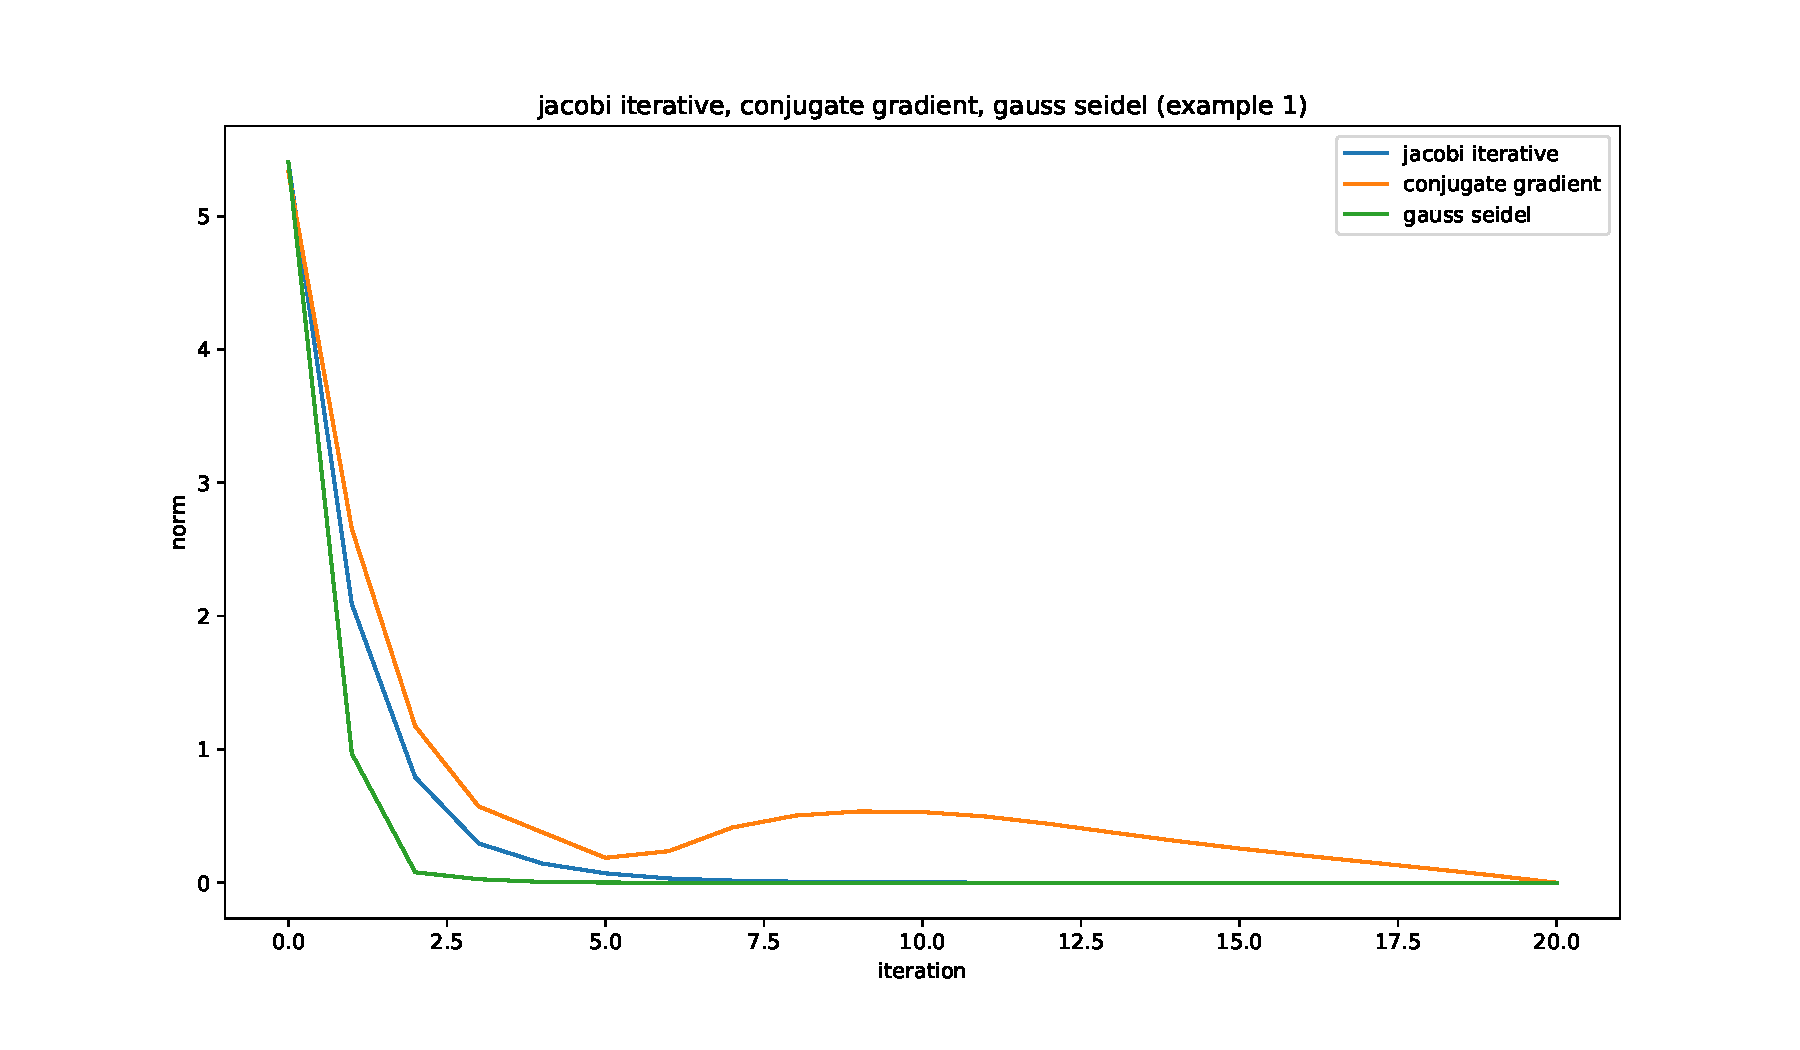
\includegraphics[width=.9\textwidth]{1}
\caption{$\norm{x - x^{(k)}}$ vs. iterations $k$ of each Iterative Method for Example 1}
\label{fig:1}
\end{figure}

\subsection{Example 2}
\begin{figure}[H]
\centering
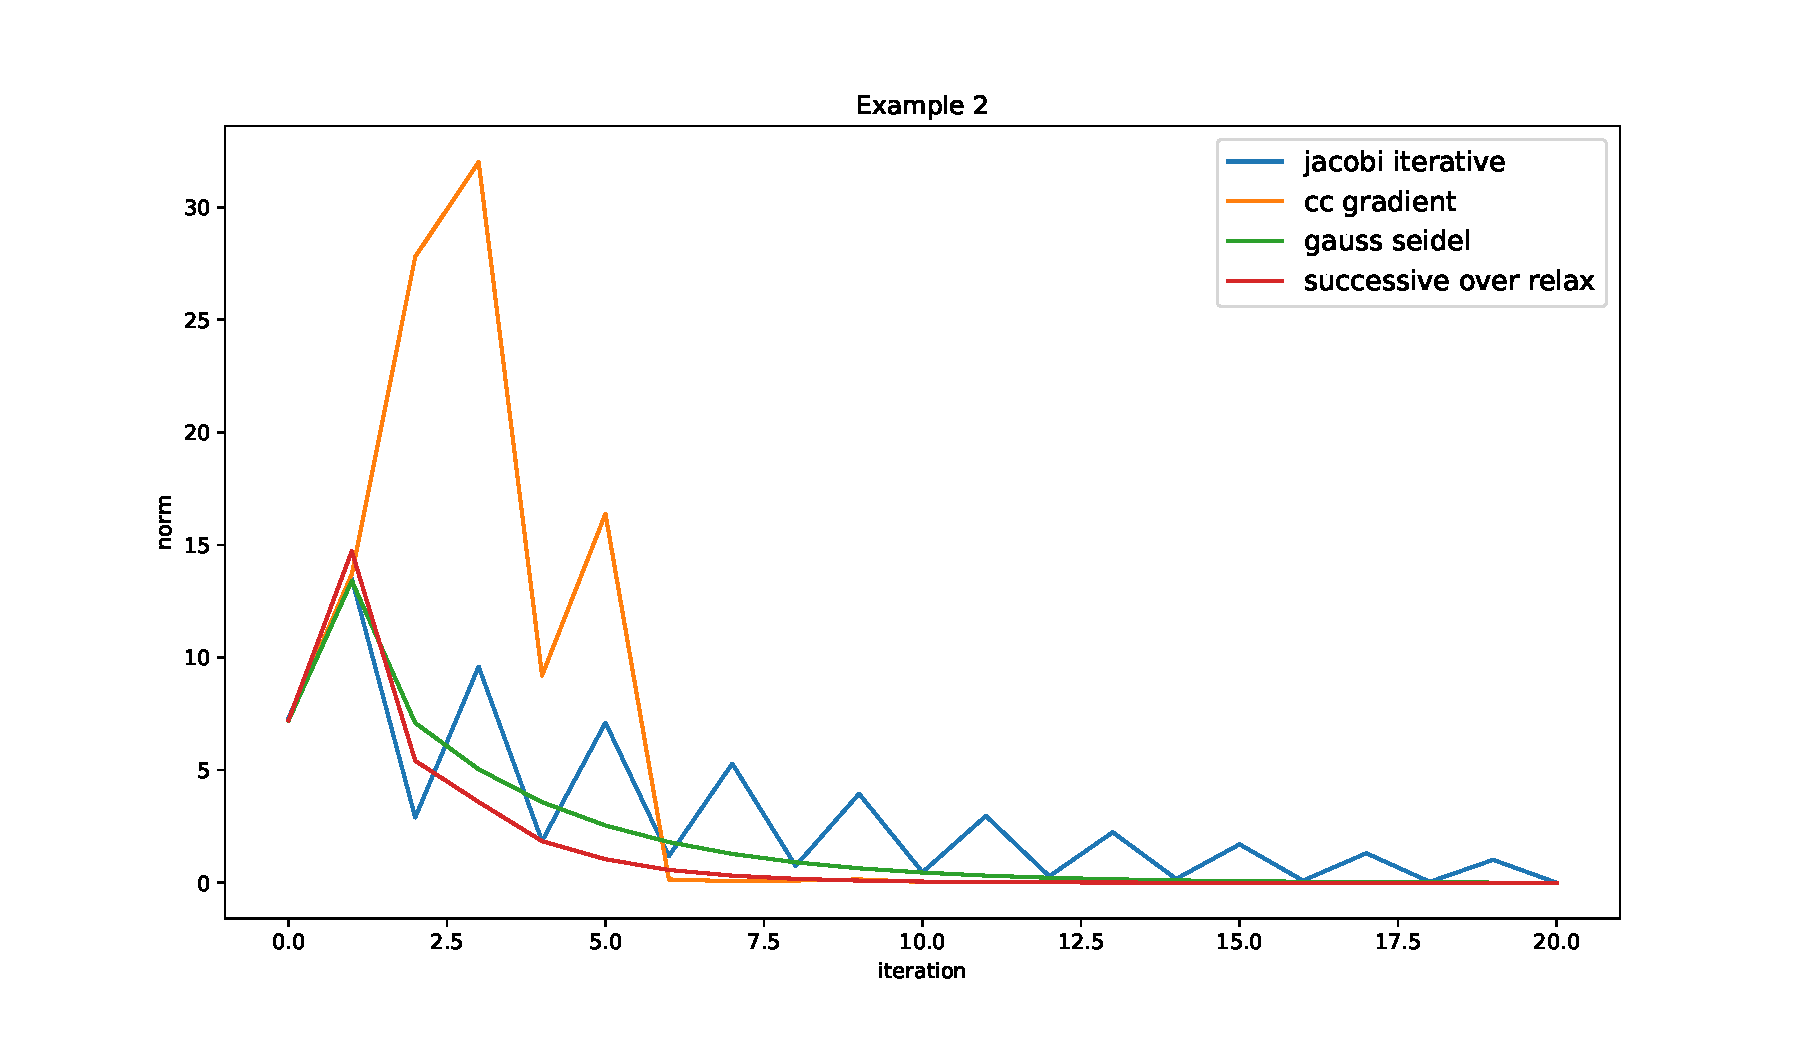
\includegraphics[width=.9\textwidth]{2}
\caption{$\norm{x - x^{(k)}}$ vs. iterations $k$ of each Iterative Method for Example 2}
\label{fig:2}
\end{figure}

\subsection{Example 3}
\begin{figure}[H]
\centering
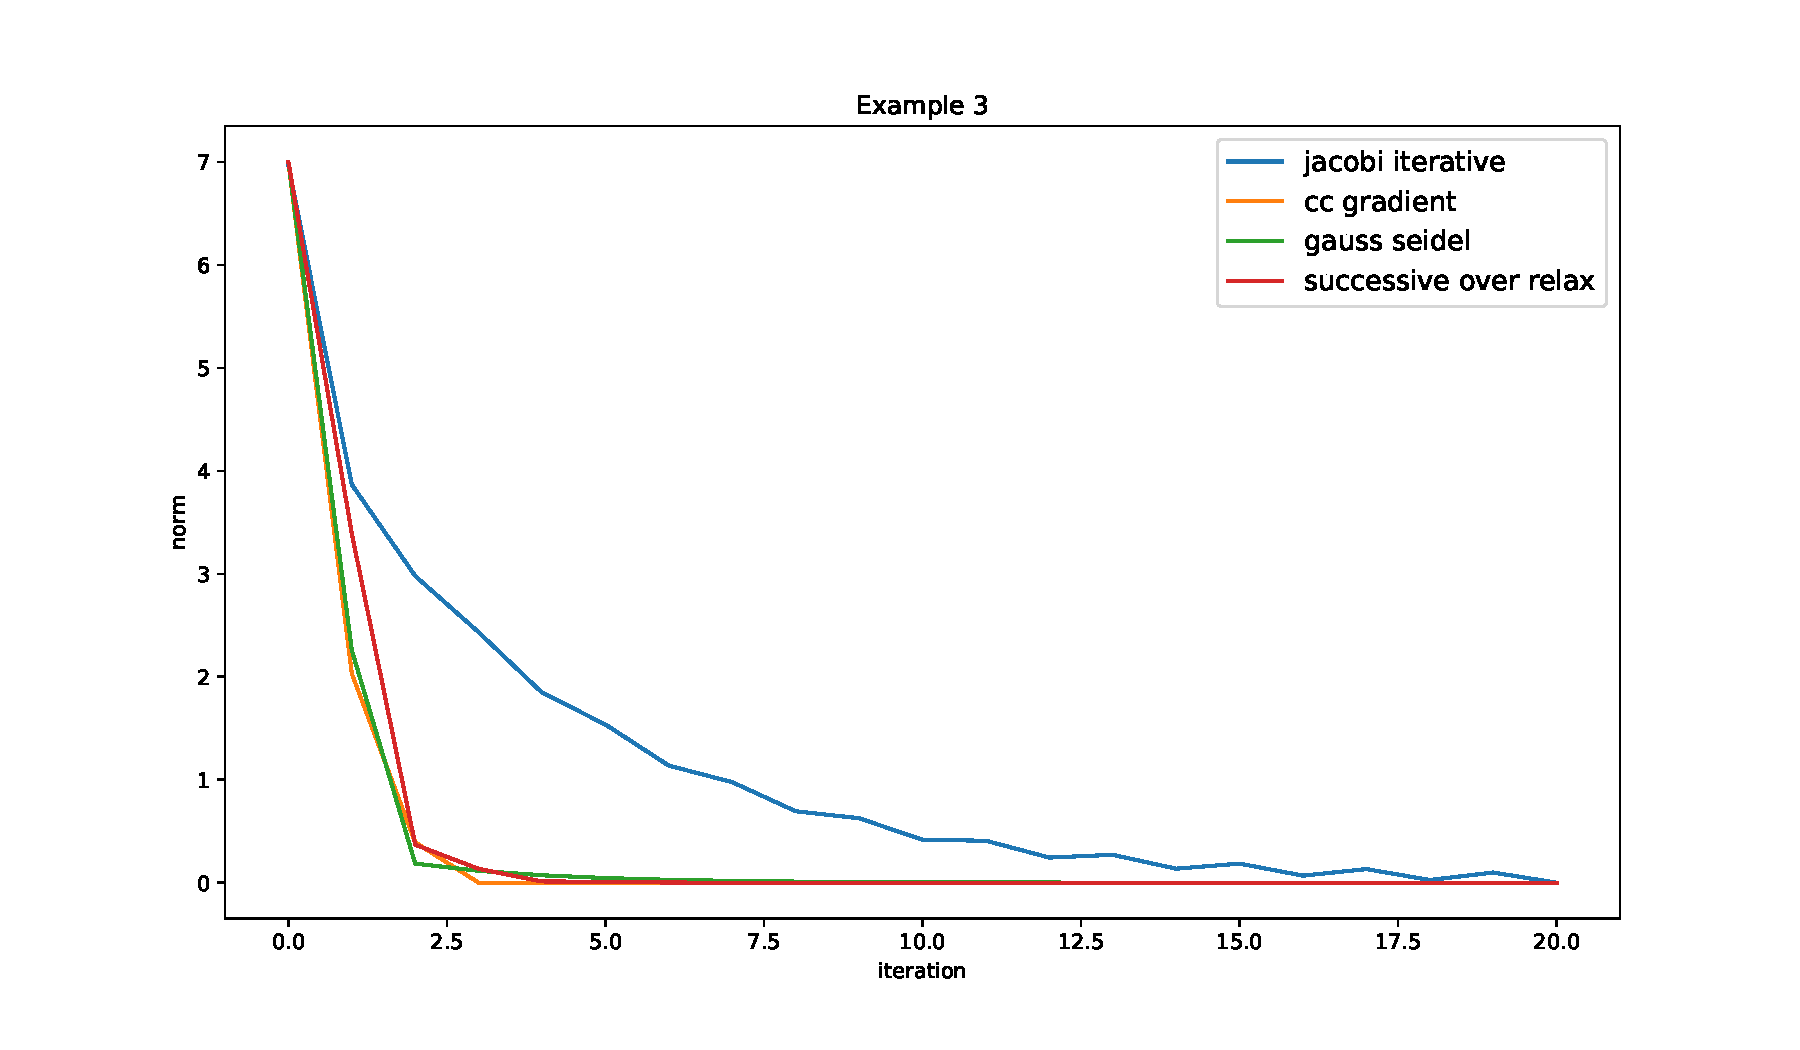
\includegraphics[width=.9\textwidth]{3}
\caption{$\norm{x - x^{(k)}}$ vs. iterations $k$ of each Iterative Method for Example 3}
\label{fig:3}
\end{figure}

\subsection{Example 4}
\begin{figure}[H]
\centering
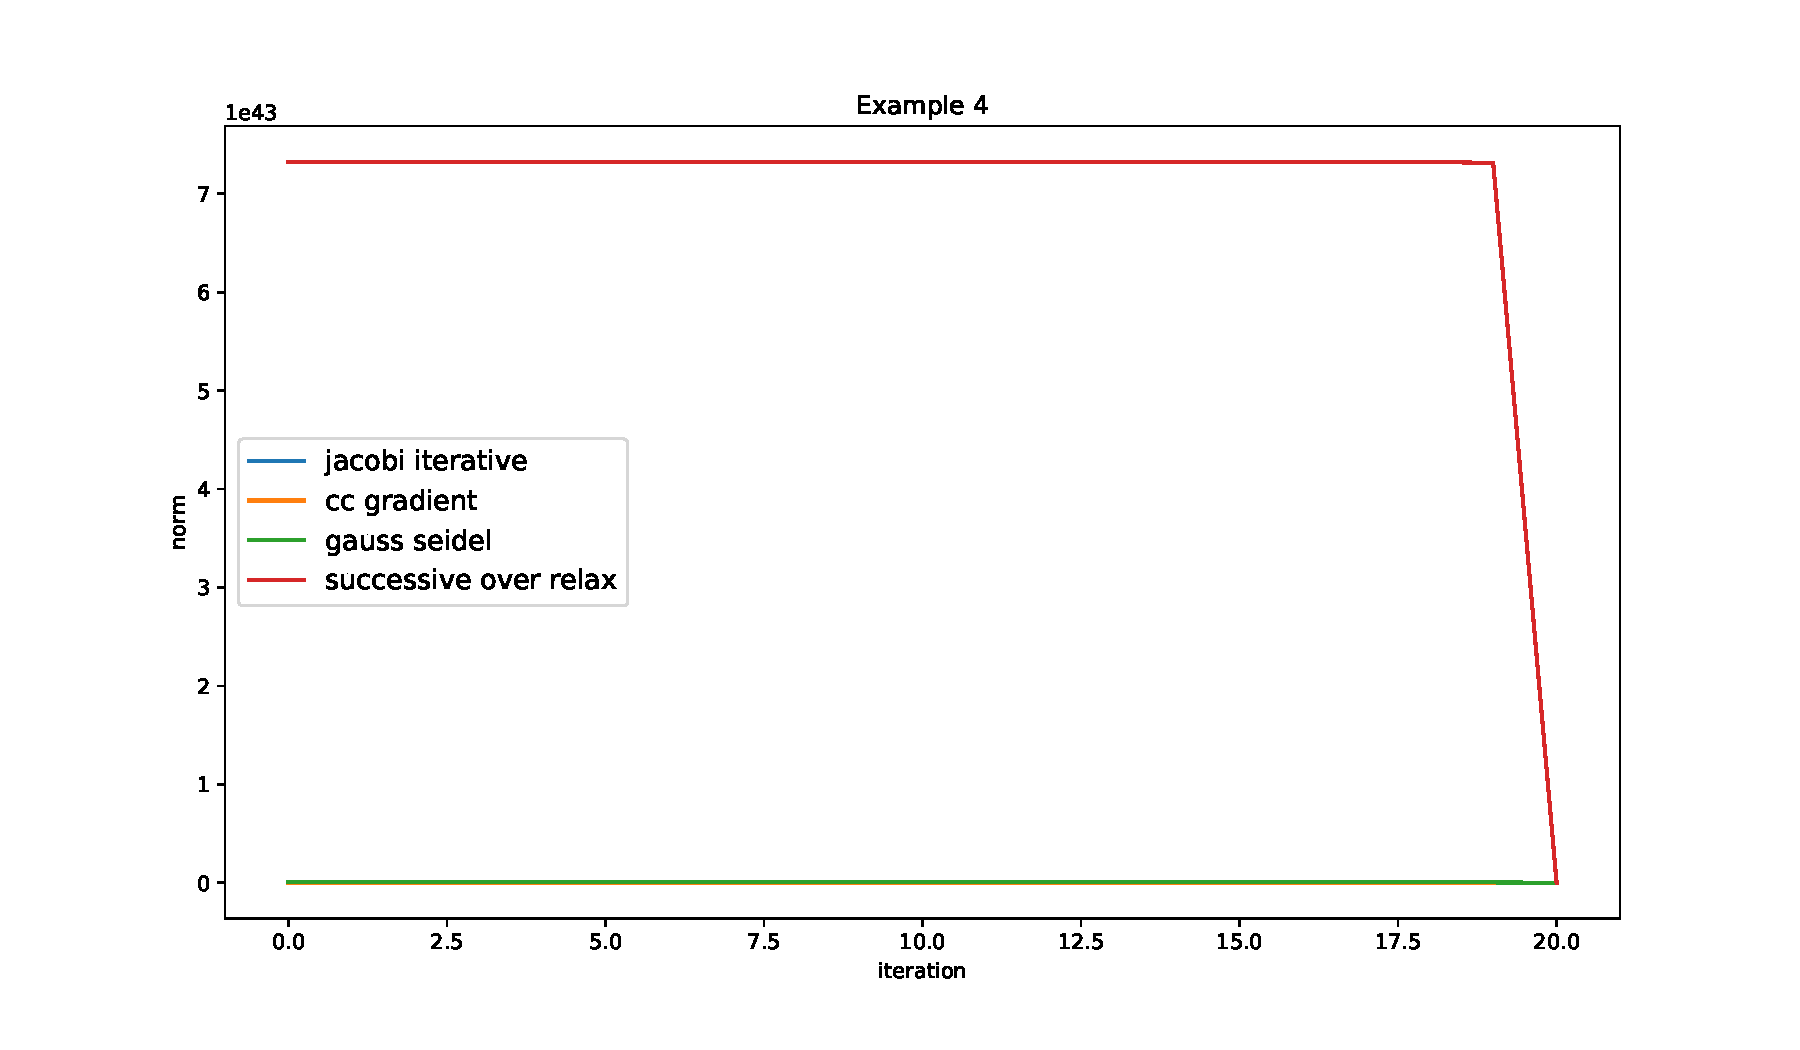
\includegraphics[width=.9\textwidth]{4}
\caption{$\norm{x - x^{(k)}}$ vs. iterations $k$ of each Iterative Method for Example 4}
\label{fig:rk4_predictor_ab4_1}
\end{figure}

\section{Discussion}
\subsection{Gaussian Elimination and Iterative Refinement}
Throughout four examples that we have tried, Gaussian elimination with variants of pivoting performed well on all of them. Solutions for these examples were computed quite quickly with very minor errors due to rounding. Though if we were to apply it on higher dimensional systems present in real life, both the computing time and precision would be a lot worse. One advantage seen of Gaussian Elimination over Iterative Methods, is that it does not require the coefficient matrix $A$ to be nice and can precisely compute the solution over any matrix given to it.

\begin{center}
	\captionof{table}{Gaussian Elimination on Example 4} \label{tab:title}
    \begin{tabular}{||c|c|c|c||}
        \hline
        Estimated & 1.0000000000001614 & 1.0 &  0.9999999999999687 \\ [.25em]
        \hline\hline
        Actual & 1.0 & 1.0 & 1.0 \\ [.25em]
        \hline
    \end{tabular}
\end{center}

Introducing partial pivoting and scaled partial pivoting to Gaussian Elimination improved precision on some of the examples. For example four, while partial pivoting did not improve improve accuracy too much, scaled partial pivoting improved accuracy by a considerable amount considering the rounding accuracy into account. In general, partial pivoting only requires about $\frac{n^2}{2}$ more boolean comparisons which has marginal affect on computational time; however scaled partial pivoting increases computational cost noticeably by adding $O(\frac{n^3}{3})$ and $\frac{n(n+1)}{2} - 1$ divisions which cost more than simple comparisons. But if computing time is important, Iterative Methods can be used that achieve reasonable precision in linear number of comparisons and arithmetic operations. Considering most real world systems are not nice, for high precision Gaussian elimination with scaled partial pivoting is advisable.

\begin{center}
	\captionof{table}{Gaussian Elimination with Partial Pivoting on Example 4} \label{tab:title}
    \begin{tabular}{||c|c|c|c||}
        \hline
        Estimated & 1.0000000000001614 & 1.0 &  1.0000000000000264 \\ [.25em]
        \hline\hline
        Actual & 1.0 & 1.0 & 1.0 \\ [.25em]
        \hline
    \end{tabular}
\end{center}

\begin{center}
	\captionof{table}{Gaussian Elimination with Scaled Partial Pivoting on Example 4} \label{tab:title}
    \begin{tabular}{||c|c|c|c||}
        \hline
        Estimated & 1.0000000000000002 & 1.0 &  0.9999999999999999 \\ [.25em]
        \hline\hline
        Actual & 1.0 & 1.0 & 1.0 \\ [.25em]
        \hline
    \end{tabular}
\end{center}

Though when precision is of utmost importance, Iterative Refinement takes the cake. For each problem by applying Gaussian Elimination first, it was able to refine the rounding errors completely up to the precision we ran our computations in. In our tests, it refined Gaussian Elimination enough to give exact solutions for the problems without a noticeable increase in running time. Though generally, Iterative Refinement acquires highest precision it can by applying a given algorithm on a residual problem multiple times and creates a substantial increase in computational cost but not overly so. In the end, the ability of Iterative Refinement to give exact answer up to the t-arithmetic digits makes it worthwhile when such precision is necessary.

\begin{center}
	\captionof{table}{Iterative Refinement of Gaussian Elimination on Example 4} \label{tab:title}
    \begin{tabular}{||c|c|c|c||}
        \hline
        Estimated & 1.0 & 1.0 &  1.0 \\ [.25em]
        \hline\hline
        Actual & 1.0 & 1.0 & 1.0 \\ [.25em]
        \hline
    \end{tabular}
\end{center}

\subsection{Iterative Methods}
For examples 1 and 4, we plotting the first 30 iterations to see the behaviors of each of the methods, and it seems like they all have surprisingly similar lack of stability in the same direction and magnitude. In example 1, all methods converge onto the same error. In example 4, PCG stays below 0, while the rest seem to increase at a linear rate, although Gauss Seidel increases at a much faster rate than the others.\\

\noindent For examples 2 and 3, we set the x axis to span 2 more than the method that converges first. In example 2, we see that although PCG has the most fluctuations, it converges the fastest at 4 iterations. Jacobi method zig-zags along, getting closer and closer until eventually converging the slowest at iteration 52.\\

\noindent One interesting note about is that the methods that have the lowest range takes the longest to converge. In example 2, PCG has a range of $[0, ~32]$, and converges the fastest, while Jacobi has $[0, ~8]$ and converges slowest. While it may seem as though PCG has more fluctuations, it is actually the case that, measured until convergence, the slower methods will experience more fluctuations.\\

\noindent In example 3, PCG converges the fasetest, however it and SOR get to almost the same value at the 4th iteration. Although SOR doesn't converge until the 8th iteration, it sits very close to the convergence number until it actually converges. After the 8th iteration, the same can be said about Gauss Seidel. \\

\noindent Overall, PCG performs best of the methods, with SOR following close behind. It is important to note, however, that each method takes relatively few iterations to get close to the convergence number. Slower methods like Jacobi's method will take a significant amount more iterations to converge, however it will have been close to the threshold for a while.

\section{Reference}
[1] R. L. Burden and J. D. Faires. Numerical Analysis 9th edition. Boston, MA: Brooks/Cole, 2011.
\end{document}
